\section{Dataset}

\subsection{Source and Structure}

The project uses MIDI files from the matched subset of the Lakh MIDI Dataset (LMD) \citep{raffelcolinLearningBasedMethodsComparing2016}, stored under \verb|data/lmd_matched/|. The MIDI files are associated with metadata and LastFM-derived tag files originating from the Lakh Pianoroll Dataset (LPD) \citep{dongMuseGANMultitrackSequential2017}. Since LPD is derived from LMD and both resources use identifiers connected to the Million Song Dataset \citep{Bertin-Mahieux2011}, the metadata can be aligned through the shared track/music identifiers.

The genre report is used as the basis for subset selection and train/validation/test split construction. It is stored at \path{data_reports/genre_dist.csv} and contains an \verb|id| column, a \verb|midi_path| column, and binary tag columns such as \verb|pop|, \verb|rock|, \verb|electronic|, \verb|jazz|, and decade-related labels. These tags are treated as weak, multi-label genre descriptors rather than as mutually exclusive ground-truth genre classes.

LastFM\footnote{\url{https://www.last.fm/api}} tags were selected because they provide a more direct track-level annotation signal for the MIDI-associated identifiers available in this repository. In contrast, MusicBrainz\footnote{\url{https://musicbrainz.org/doc/MusicBrainz_Database}}-derived metadata would require a less direct mapping through artist-level or release-level information. This distinction is important because a single artist may span multiple styles or genres over time. Therefore, the LastFM-based tags provide a more appropriate basis for track-level dataset filtering and split balancing, although they remain noisy user-derived labels.

The current split report records 36,199 candidate MIDI rows, of which 35,979 are valid after parsing and 220 are rejected due to parse errors. A sampled subset of 2,000 MIDI rows is stored in \verb|data_reports/sampled_subset.txt|. These 2,000 rows correspond to 1,230 unique music IDs, confirming that some songs have multiple MIDI representations. The subset is split using an 80\%/10\%/10\% train/validation/test ratio with random seed 42, as shown in Table~\ref{tab:splits}. The test set is held out from training and model selection and is intended for final generation-based evaluation across selected models.

\begin{table}[htbp]
	\centering
	\begin{tabular}{lrr}
		\toprule
		Split      & MIDI files & Music IDs \\
		\midrule
		Train      & 1600       & 1040      \\
		Validation & 200        & 86        \\
		Test       & 200        & 104       \\
		\bottomrule
	\end{tabular}
	\caption{Current train/validation/test split sizes stored in \texttt{data\_reports/splits/}, including unique music IDs per split.}
	\label{tab:splits}
\end{table}

\subsection{Current Dataset Statistics}

The split report uses 27 tag columns for sampling and reporting:
\begin{quote}
	\small\raggedright
	\texttt{00s}, \texttt{60s}, \texttt{70s}, \texttt{80s}, \texttt{90s}, \texttt{acoustic}, \texttt{alternative}, \texttt{american}, \texttt{blues}, \texttt{british}, \texttt{classic}, \texttt{country}, \texttt{electro}, \texttt{electronic}, \texttt{electronica}, \texttt{folk}, \texttt{funk}, \texttt{guitar}, \texttt{hardcore}, \texttt{instrumental}, \texttt{jazz}, \texttt{metal}, \texttt{piano}, \texttt{pop}, \texttt{punk}, \texttt{rock}, and \texttt{techno}.
\end{quote}
The most frequent labels in the selected subset are \verb|pop|, \verb|rock|, \verb|80s|, \verb|90s|, \verb|classic|, \verb|alternative|, \verb|electronic|, and \verb|american|, as shown in Figure~\ref{fig:genre_distro_prec_dataset}. Because the tags are multi-label, the label counts are not mutually exclusive.

Instrument summaries are also computed for descriptive analysis and split diagnostics. The most common instrument-related label is drums, followed by several General MIDI program labels such as Acoustic Grand Piano, Electric Bass (finger), String Ensemble 1, and Acoustic Guitar (steel), as shown in Figure~\ref{fig:instruments_distro_dataset}. These instrument labels are used for split balancing and diagnostic reporting, but they are not currently used as explicit conditioning inputs to the xLSTM model.

\begin{figure}[htbp]
	\centering
	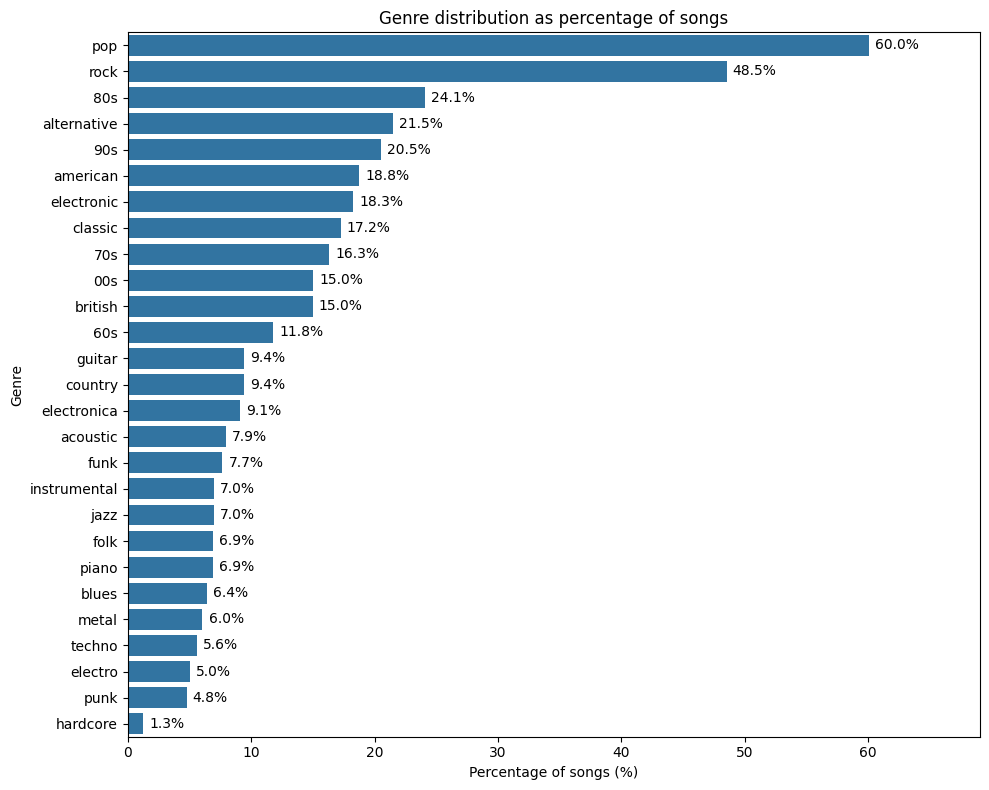
\includegraphics[width=0.75\textwidth]{figures/genre_distro_prec_dataset.png}
	\caption{Genre-label distribution based on LastFM-derived labels and track/music IDs rather than raw MIDI-file counts. This avoids over-representing songs that have multiple MIDI versions. Labels are multi-label and therefore non-exclusive.}
	\label{fig:genre_distro_prec_dataset}
\end{figure}

\begin{figure}[htbp]
	\centering
	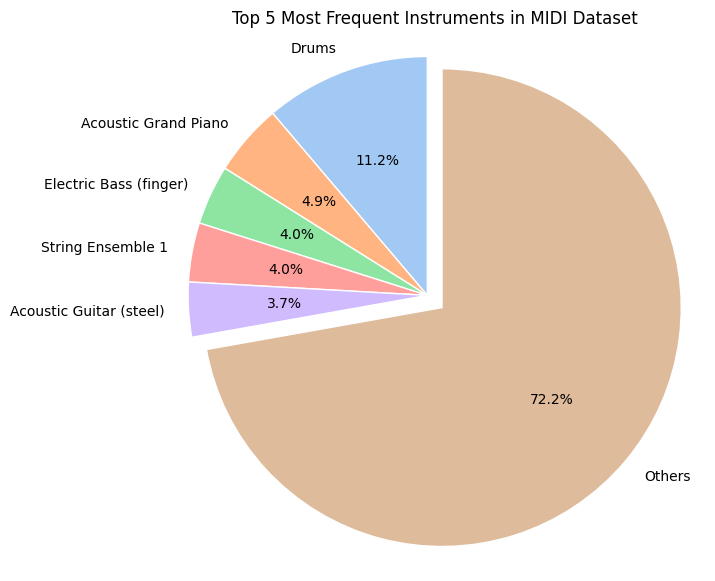
\includegraphics[width=0.5\textwidth]{figures/instruments_distro_dataset.png}
	\caption{Instrument distribution computed with the \texttt{pretty\_midi} library \citep{raffelINTUITIVEANALYSISCREATION} over the LastFM-filtered MIDI dataset. In total, 35,979 MIDI files were parsed successfully, while 220 files could not be read.}
	\label{fig:instruments_distro_dataset}
\end{figure}

\subsection{Split Construction and Leakage Controls}

The split construction code analyzes MIDI content with \verb|miditoolkit|\footnote{\url{https://github.com/YatingMusic/miditoolkit}} and computes the same PPQ-independent note-content signature used by the preprocessing code. Before the signature is computed, drum pitches are remapped to a coarse General MIDI drum map and empty tracks are removed. The signature hashes sorted note tuples containing the non-drum program number, drum flag, mapped pitch, quantized onset, and quantized duration. It is therefore designed to remove exact or near-exact file duplicates under small timing-grid and PPQ differences, but it is not a general musical near-duplicate detector: transpositions, arrangement changes, different program assignments, and larger timing or duration changes can still produce different signatures.

The current split report records 35,979 valid rows before deduplication. The first deduplication pass operates within each music ID and removes 7,897 duplicate MIDI representations, leaving 28,082 rows. The second pass groups by signature across the full candidate pool and removes 11,876 additional duplicate rows, all from 6,065 cross-ID duplicate clusters, leaving 16,206 deduplicated candidate rows. This global pass is important because identical MIDI content can appear under different metadata IDs and would not be caught by music-ID grouping alone. Algorithm~\ref{alg:dataset_split_construction} summarizes the complete construction procedure.

\begin{algorithm}[htbp]
	\caption{Deduplicated and leakage-aware split construction}
	\label{alg:dataset_split_construction}
	\DontPrintSemicolon
	\KwIn{Genre CSV with music IDs, MIDI paths, and multi-label genre tags}
	\KwOut{Sampled subset, train/validation/test split lists, and \texttt{split\_report.json}}
	Read candidate rows from \texttt{genre\_dist.csv} and resolve each MIDI path\;
	Parse each MIDI file and reject invalid or empty files\;
	Extract genre labels, top instrument labels, note counts, and the normalized content signature\;
	Group rows by music ID and keep one deterministic representative for each duplicate signature within the same ID\;
	Group the remaining rows globally by content signature and keep one deterministic representative for each duplicate signature across all IDs\;
	Select the requested 2,000-row subset from the deduplicated pool with multilabel-aware assignment over genre and instrument labels\;
	Group selected rows by music ID and assign those groups to train, validation, and test splits using the requested 80\%/10\%/10\% ratio\;
	Optionally refine the split assignment with deterministic local moves and swaps that reduce the genre/instrument JSD objective without increasing the size penalty\;
	Verify that no music ID appears in more than one split and write the output files\;
\end{algorithm}

Algorithm~\ref{alg:music_id_split_assignment} expands the split-assignment step. The splitter treats each music ID as one assignment unit, so the optimization is allowed to move complete ID groups only, not individual MIDI rows from the same song.

\begin{algorithm}[htbp]
	\caption{Music-ID grouped split assignment}
	\label{alg:music_id_split_assignment}
	\DontPrintSemicolon
	\KwIn{Deduplicated selected rows, split ratios, random seed, and refinement settings}
	\KwOut{Train, validation, and test row lists}
	Group selected rows by music ID\;
	For each music-ID group, compute its row count and aggregated genre/instrument label counts\;
	Convert the requested ratios into integer split-size targets\;
	Sort groups by rare-label priority, group size, and deterministic seed-based tie breaks\;
	\ForEach{music-ID group in sorted order}{
		Score each split by target overflow, size deviation, and label-count deviation\;
		Assign the full group to the lowest-cost split\;
	}
	Compute the initial objective from mean pairwise genre JSD, mean pairwise instrument JSD, and split-size penalty\;
	\If{refinement is enabled}{
		\ForEach{refinement iteration}{
			Try deterministic single-group moves that improve the objective without increasing size penalty\;
			If no move is accepted, try deterministic pairwise swaps between split groups\;
			Stop when no improving move or swap is found\;
		}
	}
	Expand the final music-ID group assignments back to MIDI rows\;
	Check that no music ID appears in more than one split\;
\end{algorithm}

Subset selection is performed after these deduplication passes. The final train/validation/test assignment is then made at the music-ID level for the selected rows, so any remaining multiple MIDI representations of the same identified song stay in the same split. The current split report records no train-validation, train-test, or validation-test ID overlap, indicating that exact music-ID leakage is absent in the constructed split. Together, global signature deduplication and ID-level split assignment reduce exact-content and same-ID leakage, but they do not rule out all possible musical similarity leakage from covers, alternate arrangements, or metadata errors.

The split quality is additionally diagnosed using pairwise Jensen--Shannon divergence (JSD) \citep{lin1991divergence} between train, validation, and test label distributions, computed with SciPy's distance utilities \citep{virtanenSciPy10Fundamental2020}. For genre labels, the current JSD values are 0.0206 for train-validation, 0.0097 for train-test, and 0.0154 for validation-test. For instrument labels, the corresponding values are 0.1392, 0.0889, and 0.1663. These values should be interpreted as relative split-balance diagnostics rather than as evidence that the subset is fully representative of the broader LMD distribution or free from every form of leakage.

\begin{figure}[htbp]
	\centering

	\begin{subfigure}{0.45\textwidth}
		\centering
		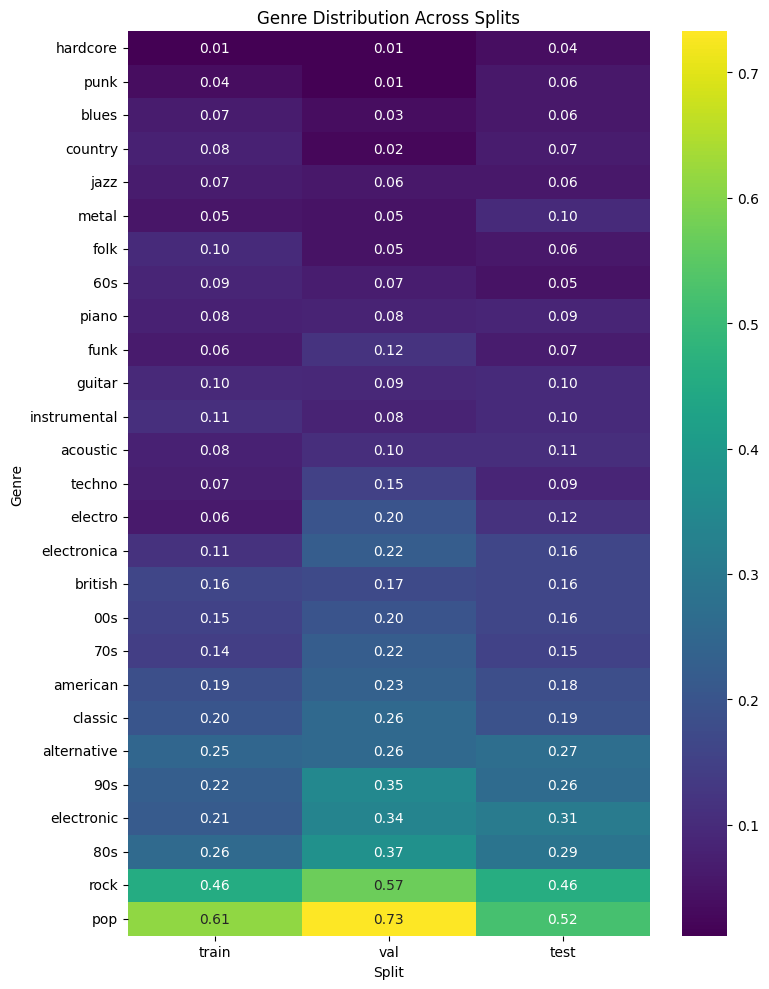
\includegraphics[width=\textwidth]{figures/genre_distro_splits.png}
		\caption{Genre-label distribution across the train, validation, and test splits.}
		\label{fig:genre_distro_splits}
	\end{subfigure}
	\hfill
	\begin{subfigure}{0.45\textwidth}
		\centering
		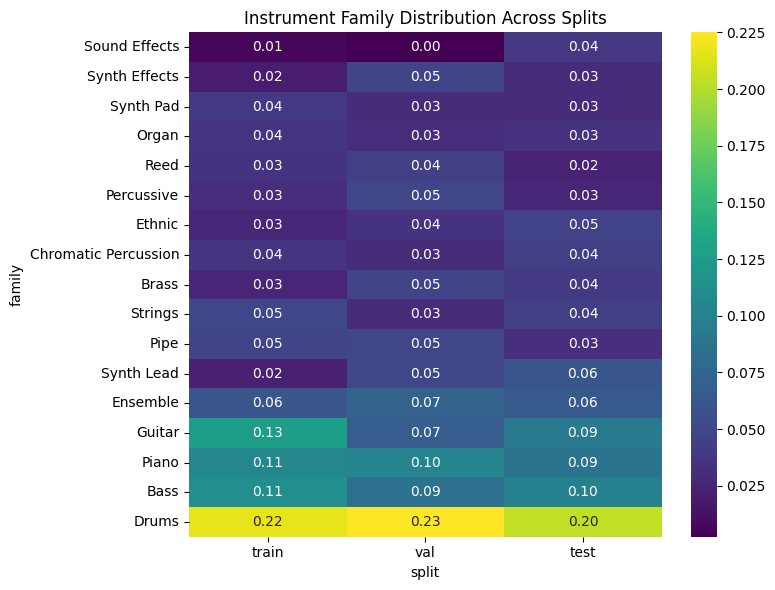
\includegraphics[width=\textwidth]{figures/instrument_families_distro_splits.png}
		\caption{Instrument-family distribution across the train, validation, and test splits.}
		\label{fig:instrument_families_distro_splits}
	\end{subfigure}

	\caption{Comparison of genre-label and instrument-family distributions across the train, validation, and test splits.}
	\label{fig:distr_splits}
\end{figure}

Figure~\ref{fig:instrument_distro_splits} provides a more fine-grained view of the same split-balance diagnostic by showing the top individual instrument labels rather than broader instrument families. This makes it easier to identify which specific General MIDI programs contribute most to any residual instrument-distribution differences across splits.

\begin{figure}[htbp]
	\centering
	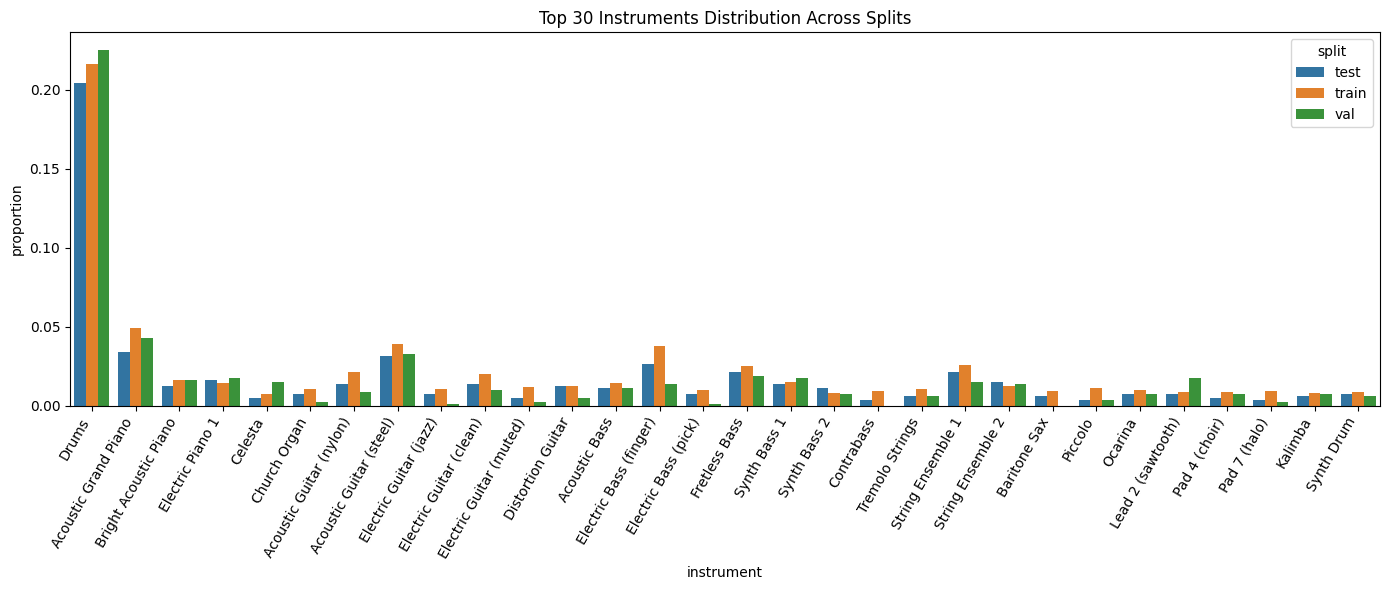
\includegraphics[width=\textwidth]{figures/instruments_distro_splits.png}
	\caption{Top 30 individual instrument-label proportions across the train, validation, and test splits.}
	\label{fig:instrument_distro_splits}
\end{figure}
